% -*- latex -*-

The Dax toolkit is built to develop a readiness for scientific data
analysis and visualizaiton at extreme scale. In particular, we address the
challenges of emerging multi- and many-core architectures. To achieve this
readiness, our project has three overarching goals.

\begin{itemize}
\item Create a toolkit that is well suited to the design of visualization
  operations with a great number of shared memory threads.
\item Develop a framework that adapts to emerging processor and compiler
  technologies.
\item Design multi-purpose algorithms that can be applied to a variety of
  visualization operations.
\end{itemize}

This chapter provides the broad design and high-level features of the Dax
toolkit that makes these goals a reality.

\section{General Approach}
\label{sec:GeneralApproach}

The Dax toolkit is designed to provide a \keyterm{pervasive parallelism}
\index{pervasive~parallelism} throughout all its visualization algorithms,
meaning that the algorithm is designed to operate with independent
concurrency at the finest possible level throughout. The Dax toolkit
provides this pervasive parallelism by providing a programming constructs
called a \keyterm{worklet}, \index{worklet} which operates on a very fine
granularity of data.  The worklets are designed as serial components, and
the Dax toolkit handles whatever layers of concurrency are necessary,
thereby removing the onus from the visualization algorithm developer.

A worklet is essentially a small functor \index{functor} or kernel
\index{kernel} designed to operate on a small element of data. (The name
``worklet'' means a small amount of work. We mean small in this sense to be
the amount of data, not necessarily the amount of instructions performed.)
The worklet is constrained to contain a serial and stateless
function. These constraints form three critical purposes. First, the
constraints on the worklets allow the Dax toolkit to schedule worklet
invocations on a great many independent concurrent threads and thereby
making the algorithm pervasively parallel. Second, the constraints allow
the Dax toolkit to provide thread safety. By controlling the memory access
the toolkit can insure that no worklet will have any memory collisions,
false sharing, or other parallel programming pitfalls. Third, the
constraints encourage good programming practices. The worklet model
provides a natural approach to visualization algorithm design that also has
good general performance characteristics.

This approach mirrors that of Baker \etal\scite{Baker2010}.  Both
approaches use C++ templating to generically apply functors in parallel to
vectors of data.  Where the Dax toolkit significantly differs from that of
Baker's is in that we are more focused on the computational geometry
problems related to scientific visualization and data analysis. Where Baker
provides a simple mapping mechanism onto a vector, our system is designed
to provide a variety of parallel scheduling operations.  These result in
worklet types that get scheduled in different ways.  Each worklet type has
a different set of capabilities. The types of worklets and their functions
is documented in Section~\ref{sec:CreatingWorklets}. These, along with
customized scheduling operations, provide reusable communicative operations
that can be applied to many visualization algorithms.

Worklets also provide additional functionality beyond the typical functor
by having flexibility in their call structure. Worklets are self describing
in that they provide signatures \index{signature} specifying the type and
meaning of input and output arguments. This functionality is described in
Section~\ref{sec:GenericScheduling}.


\section{Structure of Dax Framework}
\label{sec:StructureOfDaxFramework}

The Dax toolkit allows users to design algorithms that are run on massive
amounts of threads. These algorithms are embedded in worklets
\index{worklet} and can be run on a number of devices. However, the Dax
toolkit also allows users to interface to appliations, define data, and
invoke algorithms that they have written or are provided otherwise.

These two modes represent significantly different operations on the
data. As explained in Section~\ref{sec:GeneralApproach}, the operating code
in a worklet is constrained to access only a small portion of data that is
provided by the framework. Conversely, code that is building the data
structures needs to manage the data in its entirety, but has no reason to
perform computations on any particular element.

Consequently, the Dax toolkit is divided into two \keyterm{environments}
\index{environments} that handle each of these use cases. Each environment
has its own API, and direct interaction between the environments is
disallowed. The environments are as follows.

\begin{description}
\item[Execution Environment] \index{execution~environment} This is the
  environment in which worklets are executed. The API for this environment
  provides work for one element with convienient access to information such
  as connectivity and neighborhood as needed by typical visualization
  algorithms. Code for the execution environment is designed to always
  execute on a very large number of threads.
\item[Control Environment] \index{control~environment} This is the
  environment that is used to interface with applications, interface with
  I/O devices, and schedule parallel execution of the worklets. The
  associated API is designed for users that want to use the Dax toolkit to
  analyze their data using provided or supplied worklets. Code for the
  control environment is designed to run on a single thread (or one single
  thread per process in an MPI job).
\end{description}

These dual programming environments are partially a convenience to isolate
the application from the excution of the worklets and are partially a
necessity to support GPU languages with host and device environments. The
control and execution environments are logically equivalent to the host and
device environments, respectively, in CUDA\lcite{CUDA} and other associated
GPU languages.

\begin{figure}
  \centering
  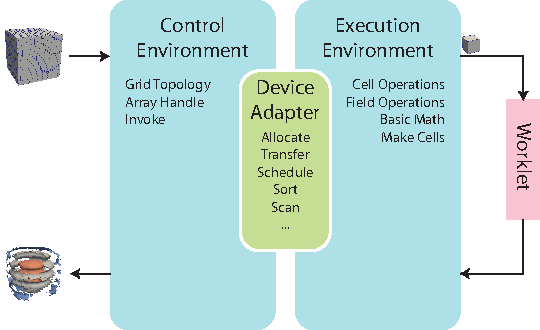
\includegraphics[width=4in]{images/DaxDiagram}
  \caption{Diagram of the Dax framework.}
  \label{fig:DaxDiagram}
\end{figure}

Figure~\ref{fig:DaxDiagram} displays the relationship between the control
and execution environment. They typical workflow when using the Dax toolkit
is that first the control thread establishes a data set in the control
environment and then invokes a parallel operation on the data using a
worklet. From there the data is logically divided into its constituent
elements, which are sent to independent invocations of the worklet. The
worklet invocations, being indepenent, are run on as many concurrent
threads as are supported by the device. On completion the results of the
worklet invocations are collected to a single data structure and a handle
is returned back to the control environment.


\section{Device Independence}
\label{sec:DeviceIndependence}

As multiple vendors vie to provide accelerator-type processors, a great
variance in the computer architecture exists, and we expect to encounter
further changes in the near future. Likewise, there exist multiple compiler
environments and libraries for these devices. The most popular of these
include OpenMP, CUDA, and OpenCL (although the latter does not yet support
C++ classes and templates). These compiler technologies also vary from
system to system.

To make porting among these systems at all feasible, we require a base
language support, and the language we use is C++. The majority of the code
in Dax is constrained to the standard C++ language constructs to minimize
the specialization from one system to the next.

\index{device~adapter|(}

Each device and device technology requires some level of code
specialization, and that specialization is encapsulated in a unit called a
\keyterm{device adapter}. Thus, porting the Dax toolkit to a new
architecture can be done by only adding a device adapter.

The device adapter is shown diagramatically as
the connection between the control and execution environments in
Figure~\ref{fig:DaxDiagram}. The functionality of the device adapter
comprises two main parts: a collection of parallel algorithms run in the
execution environment and a module to transfer data between the control and
execution environments.

Each device adapter is expected to implement a collection of algorithms
containing operations like parallel for, scan, sort, parallel find, stream
compact, and unique (remove duplicates). This list of operations is similar
to those suggested by Blelloch\scite{Blelloch1990} and Lo
\etal\scite{PISTON}. It is also a subset of those operations provided by
the Thrust library\lcite{Thrust}. Thrust itself provides a convenient
implementation for device adapters because it itself is portable among
devices. However, the interface to the device adapter algorithms is
independent of Thrust, and we have examples of device adapters that can be
built without Thrust. In fact, the Dax toolkit contains generic
implementations of every needed algorithm that minimally use only a
provided parallel for operation. However, it is usually more efficient to
provide specialized versions of at least sort and scan.

A device adapter also provides a module to handle the transfer of data
between the control and execution environments. Unlike other systems such
as CUDA and Thrust, which explicitly define separate arrays and copy
between them, the Dax device adapter allocates and copies data in one
monolithic operation. The advantage of this approach is that a device
adapter for a system that shares memory between the two environments (such
as with OpenMP) can perform shallow copies to share the data.

The implementation of device adapters is described in more detail in
Sections \ref{sec:DeviceAdapterTag} and
\ref{sec:DeviceAdapterAlgorithms}. The use of device adapters can be found
throughout Chapter~\ref{chap:Documentation}.

\index{device~adapter|)}


\section{Generic Memory Structures}
\label{sec:GenericMemoryStructures}

\fix{Generic array handle section of PDAC2012 paper.}

\fix{Reference to Section~\ref{sec:ArrayHandle}.}

\section{Generic Scheduling}
\label{sec:GenericScheduling}

\fix{Schedule metaprograms section of PDAC2012 paper.}

\fix{Reference to Section~\ref{sec:Scheduling}.}
